\documentclass[a4paper,12pt]{extarticle}

\usepackage[utf8x]{inputenc}
\usepackage[T1,T2A]{fontenc}
\usepackage[russian]{babel}
\usepackage{hyperref}
\usepackage{indentfirst}
\usepackage{listings}
\usepackage{color}
\usepackage{here}
\usepackage{array}
\usepackage{multirow}
\usepackage{graphicx}
\usepackage{caption}
\usepackage{subcaption}
\usepackage{chngcntr}
\usepackage{amsmath}
\usepackage{amssymb}
\usepackage{pgfplots}
\usepackage{pgfplotstable}
\renewcommand{\lstlistingname}{Программа} % заголовок листингов кода

\bibliographystyle{ugost2008ls}

\usepackage{listings}
\lstset{ %
extendedchars=\true,
keepspaces=true,
language=C++,						% choose the language of the code
basicstyle=\scriptsize,		% the size of the fonts that are used for the code
numbers=left,					% where to put the line-numbers
numberstyle=\scriptsize,		% the size of the fonts that are used for the line-numbers
stepnumber=1,					% the step between two line-numbers. If it is 1 each line will be numbered
numbersep=5pt,					% how far the line-numbers are from the code
backgroundcolor=\color{white},	% choose the background color. You must add \usepackage{color}
showspaces=false				% show spaces adding particular underscores
showstringspaces=false,			% underline spaces within strings
showtabs=false,					% show tabs within strings adding particular underscores
frame=single,           		% adds a frame around the code
tabsize=2,						% sets default tabsize to 2 spaces
captionpos=t,					% sets the caption-position to top
breaklines=true,				% sets automatic line breaking
breakatwhitespace=false,		% sets if automatic breaks should only happen at whitespace
escapeinside={\%*}{*)},			% if you want to add a comment within your code
postbreak=\raisebox{0ex}[0ex][0ex]{\ensuremath{\color{red}\hookrightarrow\space}},
texcl=true,
inputpath=fig,                     % директория с листингами
}

\usepackage[left=2cm,right=2cm,
top=2cm,bottom=2cm,bindingoffset=0cm]{geometry}

%% Нумерация картинок по секциям
\usepackage{chngcntr}
\counterwithin{figure}{section}
\counterwithin{table}{section}

%%Точки нумерации заголовков
\usepackage{titlesec}
\titlelabel{\thetitle.\quad}
\usepackage[dotinlabels]{titletoc}

%% Оформления подписи рисунка
\addto\captionsrussian{\renewcommand{\figurename}{Рисунок}}
\captionsetup[figure]{labelsep = period}

%% Подпись таблицы
\DeclareCaptionFormat{hfillstart}{\hfill#1#2#3\par}
\captionsetup[table]{format=hfillstart,labelsep=newline,justification=centering,skip=-10pt,textfont=bf}

%% Путь к каталогу с рисунками
\graphicspath{{fig/}}


\begin{document}	% начало документа

% Титульная страница
\begin{titlepage}	% начало титульной страницы

	\begin{center}		% выравнивание по центру

		\large Санкт-Петербургский Политехнический Университет Петра Великого\\
		\large Институт компьютерных наук и технологий \\
		\large Кафедра компьютерных систем и программных технологий\\[6cm]
		% название института, затем отступ 6см
		
		\huge Вычислительная математика\\[0.5cm] % название работы, затем отступ 0,5см
		\large Отчет по лабораторной работе №1\\[0.1cm]
		\large <<Сравнение точности интерполяционных полиномов>>\\[0.1cm]
		\large Вариант №5\\[5cm]

	\end{center}


	\begin{flushright} % выравнивание по правому краю
		\begin{minipage}{0.25\textwidth} % врезка в половину ширины текста
			\begin{flushleft} % выровнять её содержимое по левому краю

				\large\textbf{Работу выполнил:}\\
				\large Ламтев А.Ю.\\
				\large {Группа:} 23501/4\\
				
				\large \textbf{Преподаватель:}\\
				\large Цыган В.Н.

			\end{flushleft}
		\end{minipage}
	\end{flushright}
	
	\vfill % заполнить всё доступное ниже пространство

	\begin{center}
	\large Санкт-Петербург\\
	\large \the\year % вывести дату
	\end{center} % закончить выравнивание по центру

\thispagestyle{empty} % не нумеровать страницу
\end{titlepage} % конец титульной страницы

\vfill % заполнить всё доступное ниже пространство


\section{Цель работы}
Исследовать зависимость нормы матрицы от возмущения исходных данных.

\section{Решаемые задачи}
\begin{enumerate}

\item Составить процедуру вычисления по заданной матрице $A_{N \times N}$ матрицы \\$R = A^{-1} A - E$ и её нормы $||R|| = \max_{k} \sum_j^N |R_{jk}|$.

\item Построить матрицы A при $x_k = \frac{1 + cos(k)}{sin^2(k)}, k = 1, \dots, 4$ и $x_5 = \frac{1+cos(1)}{sin^2(1 + \varepsilon)}$, для значений $\varepsilon = 10^{-1}, 10^{-2}, 10^{-3}, \dots, 10^{-16}, 0$ и $N = 5$.

\begin{displaymath}
A=
  \begin{pmatrix}
    1 & 1 & \dots & 1 \\
    x_1 & x_2 & \dots & x_N \\
    \dots & \dots & \dots & \dots & \\
    x_1^{N-1} & x_2^{N-1} & \dots & x_N^{N-1} \\
  \end{pmatrix}
\end{displaymath}


\item  Исследовать зависимость погрешности вычисления $||R||$ от $\varepsilon$.
\end{enumerate}


\section{Ход выполнения работы}

В ходе выполнения работы было разработано программное обеспечение на языке программирования \textbf{java}, позволяющее решить поставленные задачи. Данное программное обеспечение включает в себя:
\begin{itemize}

\item Библиотеку \textbf{MatrixUtil} с функциями \textbf{decomp} и \textbf{solve}, которые содержат вызовы стандартных форсайтовских функций \textbf{decomp} и \textbf{solve}, разработанных на языке программирования \textbf{с}, из динамической библиотеки.

\item Библиотеку \textbf{Matrix}, позволяющую совершать различные действия над матрицами, в том числе, \textit{обращение, произведение, вычитание, вычисление нормы}, которые необходимы для решения поставленных задач.

 \textit{Обращение} матрицы реализовано как n итераций решения системы $\textbf{A}x = \textbf{B}$ при помощи функций \textbf{decomp} и \textbf{solve} c $\textbf{B}$ -- i-м столбцом единичной матрицы на i-й итерации и n -- порядком матрицы. Реализация представлена в листинге \ref{code:Matrix:inverted}.
 
 Реализации \textit{произведения, вычитания, вычисления нормы} представлены в листингах \ref{code:Matrix:multiply}, \ref{code:Matrix:minus} и \ref{code:Matrix:calculateNormAsMaximumAbsoluteColumnSum} соответственно.

\item Приложение, решающее поставленные задачи и использующее ранее перечисленные библиотеки (листинг \ref{code:Lab2}).

\end{itemize} 

Была исследована зависимость $||R||$ от величины $\varepsilon$, при $\varepsilon = 10^{-1}, 10^{-2}, \dots, 10^{-16}, 0$:\\[3mm]

При $\varepsilon = 10^{-1}$ -- $||R|| \simeq 9.7 \cdot 10^{-13}$.

При $\varepsilon = 10^{-2}$ -- $||R|| \simeq 4.5 \cdot 10^{-13}$.

Далее с уменьшением $\varepsilon$ постепенно возрастает значение $||R||$ и достигает $0.75$ при $\varepsilon = 10^{-15}$.

На интервале $(10^{-16}, 10^{-15})$ $||R||$ принимает значения от 2 до 5.

При $\varepsilon = 10^{-16}$ происходит резкое возрастание нормы матрицы R до 129.

При дальнейшем уменьшении $\varepsilon$ вплоть до 0 $||R||$ остается 129.\\[3mm]
   
   На рисунках \ref{pic:demo1}, \ref{pic:demo2} и \ref{pic:demo3} изображен вывод программы, иллюстрирующий наблюдения, для $\varepsilon = 10^{-2}, 10^{-6}, 10^{-10}, 10^{-15}, 10^{-16}, 0$.

\begin{figure}[H]
    \centering
    \begin{subfigure}[t]{0.5\textwidth}
        \centering
        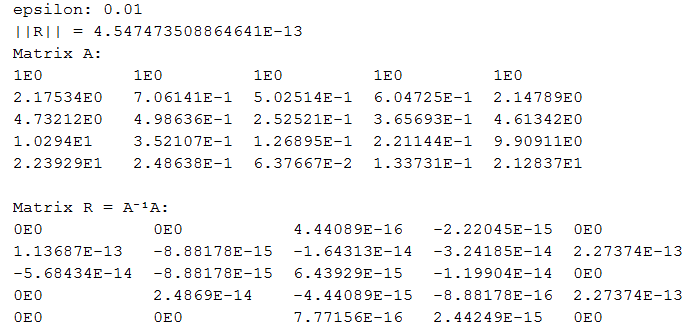
\includegraphics[height=1.60in]{2}
        \caption{при $\varepsilon = 10^{-2}$}
    \end{subfigure}%
    ~ 
    \begin{subfigure}[t]{0.5\textwidth}
        \centering
        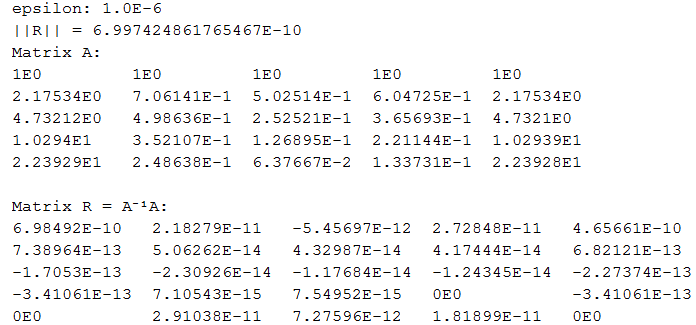
\includegraphics[height=1.60in]{6}
        \caption{при $\varepsilon = 10^{-6}$}
    \end{subfigure}
    \caption{Вывод программы}
    \label{pic:demo1}
\end{figure}

\begin{figure}[H]
    \centering
    \begin{subfigure}[t]{0.5\textwidth}
        \centering
        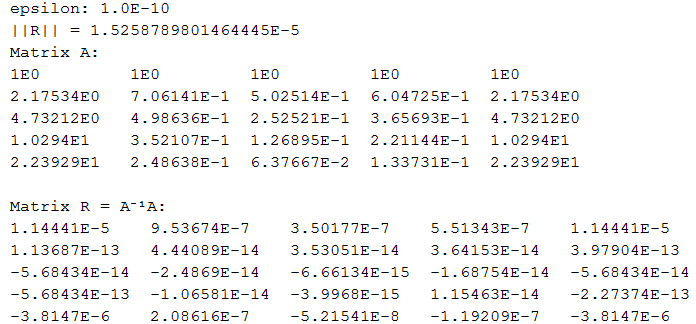
\includegraphics[height=1.60in]{10}
        \caption{при $\varepsilon = 10^{-10}$}
    \end{subfigure}%
    ~ 
    \begin{subfigure}[t]{0.5\textwidth}
        \centering
        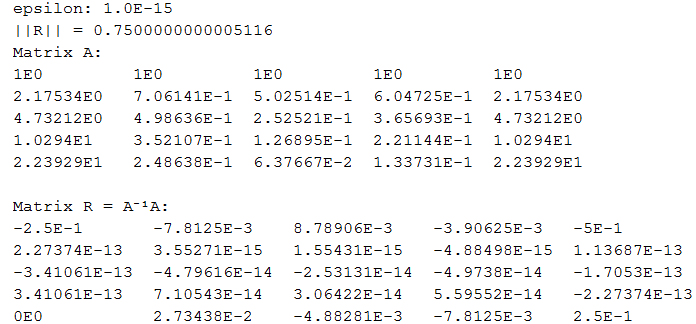
\includegraphics[height=1.60in]{15}
        \caption{при $\varepsilon = 10^{-15}$}
    \end{subfigure}
    \caption{Вывод программы}
    \label{pic:demo2}
\end{figure}

\begin{figure}[H]
    \centering
    \begin{subfigure}[t]{0.5\textwidth}
        \centering
        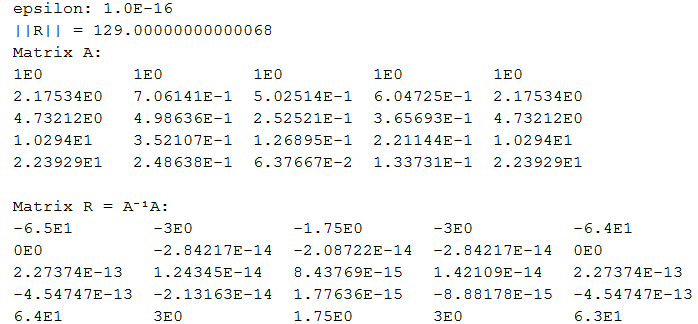
\includegraphics[height=1.60in]{16}
        \caption{при $\varepsilon = 10^{-16}$}
    \end{subfigure}%
    ~ 
    \begin{subfigure}[t]{0.5\textwidth}
        \centering
        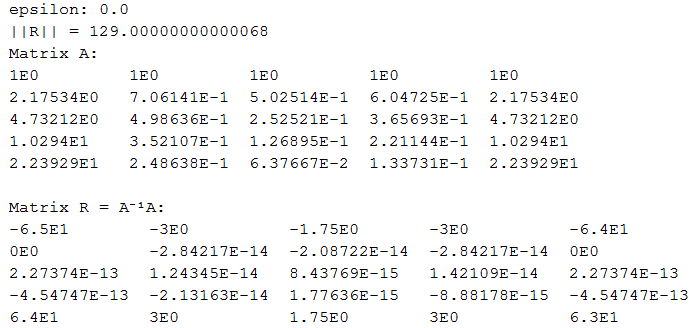
\includegraphics[height=1.60in]{0}
        \caption{при $\varepsilon = 0$}
    \end{subfigure}
    \caption{Вывод программы}
    \label{pic:demo3}
\end{figure} 

На рисунках \ref{pic:graphic1} и \ref{pic:graphic2} изображены графики зависимости нормы матрицы от $\varepsilon$ на всем интервале и на отрезке $[10^{-16}, 10^{-1}]$ соответственно.

\begin{figure}[H]
\begin{center}
	\begin{tikzpicture} [every plot/.append style={thick}]
		\begin{axis}[
			height=0.3\textheight,
			width=0.9\textwidth,
			xlabel={$\varepsilon$},
			ylabel={$||R||$},
			xlabel near ticks,
			ylabel near ticks,			
			xmax=1,
			xmin=0,
			ymax=140,
			ymin=-10,
			xmode=log,
			log basis x=10,			
			grid=major
		]
		\addplot table[x=epsilon,y=norm,col sep=comma]{data/norm_full.csv};
		\end{axis}
	\end{tikzpicture}
	\caption{Зависимость нормы матрицы R от $\varepsilon$. Полный интервал}
	\label{pic:graphic1}
\end{center}
\end{figure}

~

\begin{figure}[H]
\begin{center}
	\begin{tikzpicture} [every plot/.append style={thick}]
		\begin{axis}[
			height=0.35\textheight,
			width=0.9\textwidth,
			xlabel={$\varepsilon$},
			ylabel={$||R||$},
			xlabel near ticks,
			ylabel near ticks,
			xmax=0.2,
			xmin=1e-16,
			ymax=5.2,
			ymin=-0.2,
			xmode=log,
			log basis x=10,			
			grid=major
		]
		\addplot table[x=epsilon,y=norm,col sep=comma]{data/norm_right.csv};
		\end{axis}
	\end{tikzpicture}
	\caption{Зависимость нормы матрицы R от $\varepsilon$. Отрезок $[10^{-16}, 10^{-1}]$}
	\label{pic:graphic2}
\end{center}
\end{figure}

\section{Выводы}
В результате работы была исследована зависимость нормы матрицы R от $\varepsilon$. При $\varepsilon = 10^{-13} \dots 10^{-1}$ значение $||R||$ близко к нулю, что не противоречит здравому смыслу, так как аналитически вычисленная матрица R (\textit{нулевая}) имеет норму 0. При последовательном уменьшении $\varepsilon$ до 0 значение нормы матрицы монотонно возрастает (за исключением интервала $(10^{-16}, 10^{-15})$) и достигает предела приблизительно равного 129.

Итак, применение стандартных функций \textbf{decomp} и \textbf{solve} для получения заданной матрицы R из заданной матрицы A, заполненной числами с плавающей запятой двойной точности, целесообразно при $\varepsilon = 10^{-13} \dots 10^{-1}$.
\newpage

\section*{Приложение 1. Листинги кода}

\lstinputlisting[
	label=code:Lab2,
	caption={Lab2.java},% для печати символ '_' требует выходной символ '\'
]{../../../app/src/main/java/com/lamtev/comp_maths_labs/lab2/app/Lab2.java}
\parindent=1cm % командна \lstinputlisting сбивает параментры отступа

\newpage

\captionof{lstlisting}{Конструктор Matrix.}
\lstinputlisting[label=code:Matrix:Matrix, linerange={27-32}]{../../../matrix_lib/src/main/java/com/lamtev/comp_maths_labs/lab2/matrix_lib/Matrix.java}
\parindent=1cm

\captionof{lstlisting}{Метод Matrix::Identity.\\ Возвращает единичную матрицу указанного порядка}
\lstinputlisting[label=code:Matrix:Identity, linerange={19-25}]{../../../matrix_lib/src/main/java/com/lamtev/comp_maths_labs/lab2/matrix_lib/Matrix.java}
\parindent=1cm

\captionof{lstlisting}{Метод Matrix::inverted.\\ Возвращает обратную матрицу к данной}
\lstinputlisting[label=code:Matrix:inverted, linerange={133-158}]{../../../matrix_lib/src/main/java/com/lamtev/comp_maths_labs/lab2/matrix_lib/Matrix.java}
\parindent=1cm

\captionof{lstlisting}{Метод Matrix::multiply.\\ Возвращает матрицу, являющуюся результатом произведения данной матрицы с матрицейб переданной в качестве аргумента.}
\lstinputlisting[label=code:Matrix:multiply, linerange={108-119}]{../../../matrix_lib/src/main/java/com/lamtev/comp_maths_labs/lab2/matrix_lib/Matrix.java}
\parindent=1cm

\captionof{lstlisting}{Метод Matrix::minus.\\ Возвращает матрицу, являющуюся результатом разности данной матрицы с матрицей, переданной в качестве аргумента.}
\lstinputlisting[label=code:Matrix:minus, linerange={97-106}]{../../../matrix_lib/src/main/java/com/lamtev/comp_maths_labs/lab2/matrix_lib/Matrix.java}
\parindent=1cm

\captionof{lstlisting}{Метод
Matrix::normAsMaximumAbsoluteColumnSum.\\ Возвращает ранее вычисленную норму (максимальную абсолютную сумму елементов внутри одного столбца) матрицы.}
\lstinputlisting[label=code:Matrix:normAsMaximumAbsoluteColumnSum, linerange={78-80}]{../../../matrix_lib/src/main/java/com/lamtev/comp_maths_labs/lab2/matrix_lib/Matrix.java}
\parindent=1cm

\captionof{lstlisting}{Метод
Matrix::calculateNormAsMaximumAbsoluteColumnSum.\\ Вычисляет норму (максимальную абсолютную сумму елементов внутри одного столбца) матрицы.}
\lstinputlisting[label=code:Matrix:calculateNormAsMaximumAbsoluteColumnSum, linerange={250-263}]{../../../matrix_lib/src/main/java/com/lamtev/comp_maths_labs/lab2/matrix_lib/Matrix.java}
\parindent=1cm

\end{document}
